\begin{center}
    \captionof{figure}{Path diagrams of Generative Models with Within-Person ($\beta_1$) and Contextual Effect ($\gamma_{01}$)}
    % Top row
    \begin{minipage}[t]{.49\linewidth}
        \centering
        \begin{subfigure}[b]{\linewidth}
            \centering
            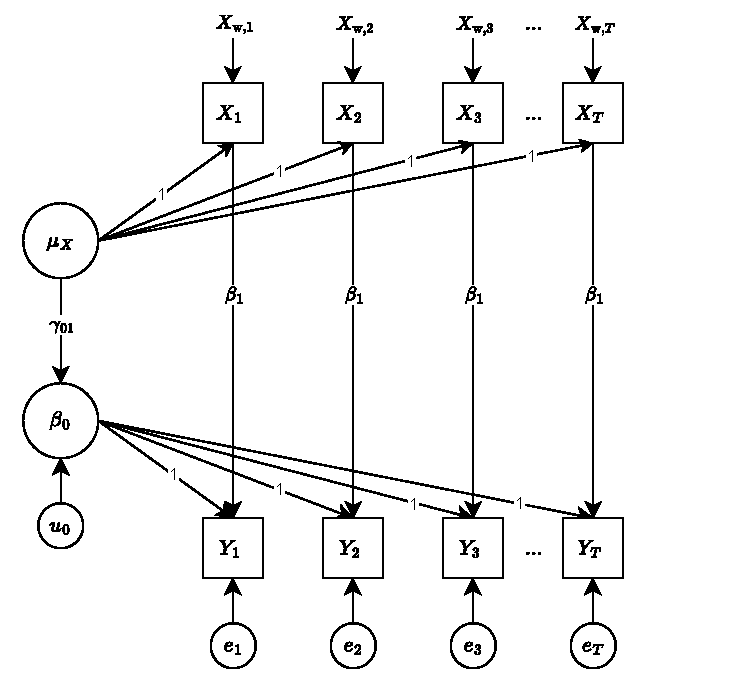
\includegraphics[height=6.5cm]{Figures/pathdiagrams-cropped-contxy.drawio.pdf}
            \caption{Continuous X and Y}\label{fig:path-contxy}
        \end{subfigure}
    \end{minipage}
    \hfill
    \begin{minipage}[t]{.49\linewidth}
        \centering
        \begin{subfigure}[b]{\linewidth}
            \centering
            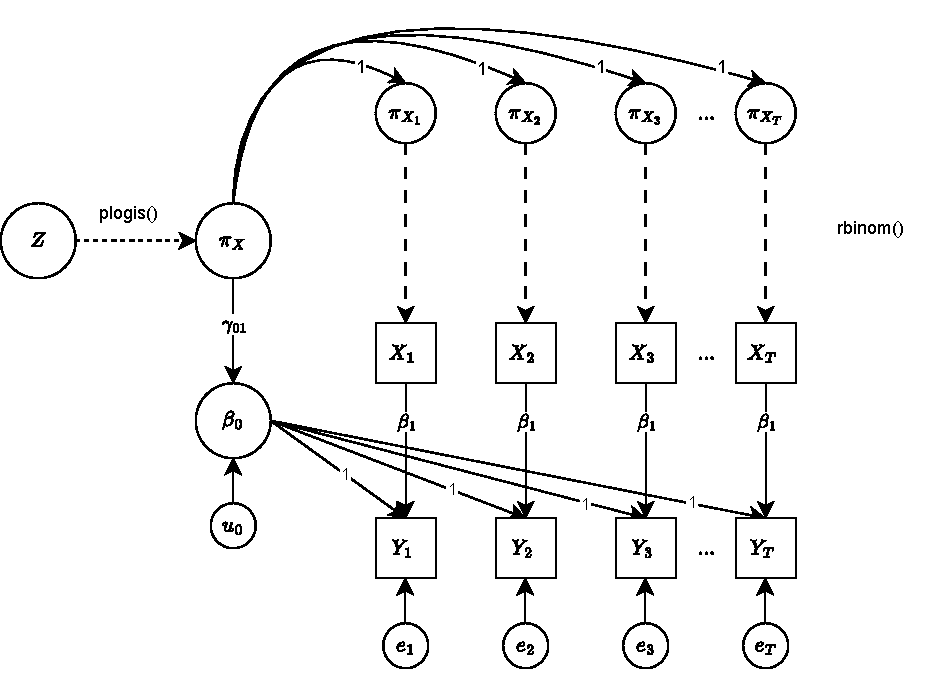
\includegraphics[height=6.5cm]{Figures/pathdiagrams-cropped-binxconty.drawio.pdf}
            \caption{Binary X and Continuous Y}\label{fig:path-binxconty}
        \end{subfigure}
    \end{minipage}

    % \vskip 1em

    % Bottom row
    \begin{minipage}[t]{.49\linewidth}
        \centering
        \begin{subfigure}[b]{\linewidth}
            \centering
            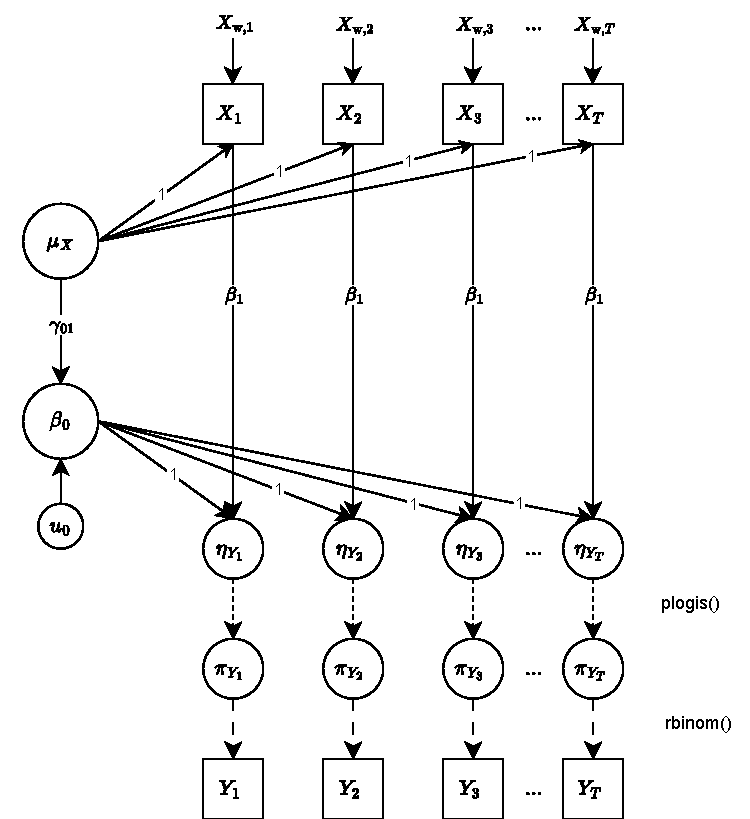
\includegraphics[height=7.5cm]{Figures/pathdiagrams-cropped-contxbiny.drawio.pdf}
            \caption{Continuous X and Binary Y}\label{fig:path-contxbiny}
        \end{subfigure}
    \end{minipage}
    \hfill
    \begin{minipage}[t]{.49\linewidth}
        \centering
        \begin{subfigure}[b]{\linewidth}
            \centering
            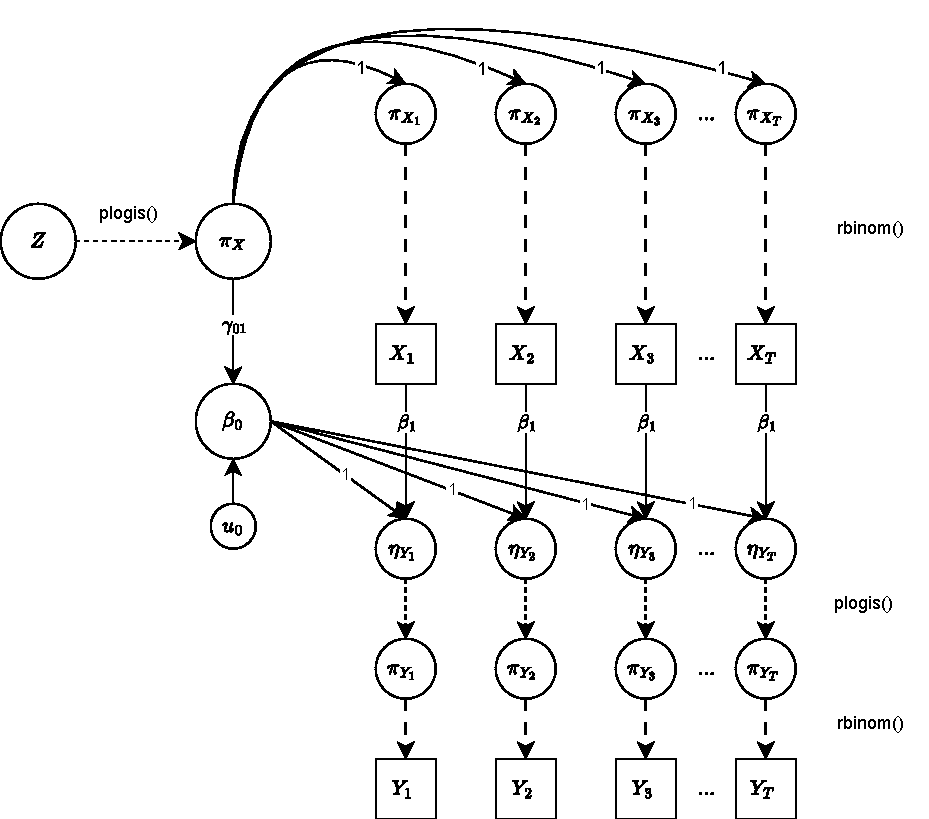
\includegraphics[height=7.5cm]{Figures/pathdiagrams-cropped-binxy.drawio.pdf}
            \caption{Binary X and Y}\label{fig:path-binxy}
        \end{subfigure}
    \end{minipage}
    \vspace{-0.5cm}
    \label{fig:path}
    \begin{flushleft}
    \begin{figurenote}
    Path diagrams of the four data-generating models, varying by predictor type $X$ (columns) and outcome type $Y$ (rows), each either continuous or binary. In all models, the outcome is regressed on the predictor, and the person-level predictor mean $\mu_X$ predicts the outcome intercept $\beta_0$, yielding a within-person slope $\beta_1$ and a contextual effect $\gamma_{01}$. Circles represent latent variables, squares observed variables. Solid arrows denote linear relations; dotted arrows indicate logit transformations (\texttt{plogis} in \texttt{R}); dashed arrows indicate Bernoulli sampling with probability $\pi$ (\texttt{rbinom} in \texttt{R}).
    
    % Path diagrams of four data generating models that vary in predictor type $X$ (column wise) and outcome type $Y$ (row wise), both of which are either continuous or binary. Models are based regressing the outcome variable on the predictor, while using the latent mean per person on the predictor $\mu_X$ to predict the intercept $\beta_{0}$ of the outcome. This results in the within-person slope $\beta_1$ and the contextual effect $\gamma_{01}$. Circles denote latent variables, squares denote observed variables, and arrows represent relationships. Solid arrows indicate linear associations, dotted arrows represent logit transformations (\texttt{plogis} in \texttt{R}), and dashed arrows indicate Bernoulli sampling with probability $\pi$ (\texttt{rbinom} in \texttt{R}).
    % Circles represent latent variables, squares represent observed variables, and arrows indicate relationships. Solid arrows denote linear associations, with a coefficient of 1 indicating a one-to-one relationship. Dotted arrows represent logit transformations (\texttt{plogis} in \texttt{R}), and dashed arrows represent Bernoulli sampling based on the probability $\pi$ (\texttt{rbinom} in \texttt{R}).
    \end{figurenote}
    \end{flushleft}
\end{center}

% \begin{center}
%     \captionof{figure}{Path diagrams of Generative Models with Within-Person ($\beta_1$) and Contextual Effect ($\gamma_{01}$)}
%     % Top row
%     \begin{minipage}[t]{.49\linewidth}
%         \centering
%         \begin{subfigure}[b]{\linewidth}
%             \centering
%             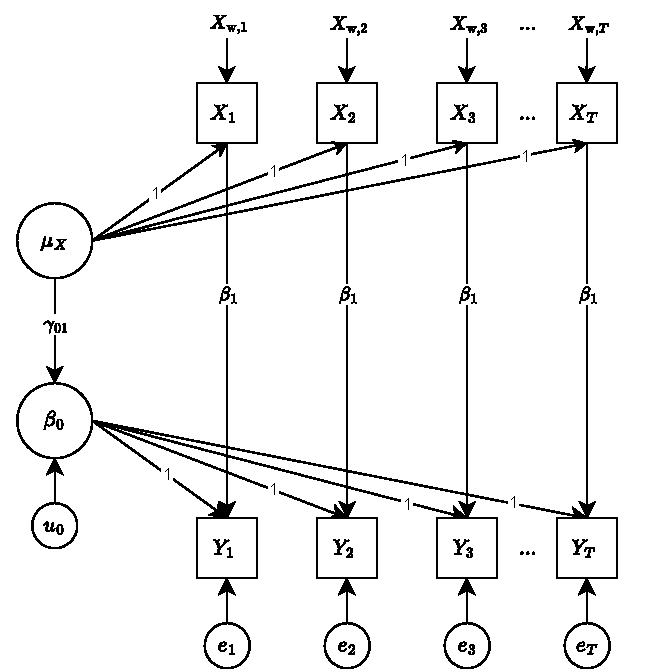
\includegraphics[width=\linewidth, height=8cm, keepaspectratio]{Figures/pathdiagrams-contxy.drawio.pdf}
%             \caption{Continuous X and Y}\label{fig:path-contxy}
%         \end{subfigure}
%     \end{minipage}
%     \hfill
%     \begin{minipage}[t]{.49\linewidth}
%         \centering
%         \begin{subfigure}[b]{\linewidth}
%             \centering
%             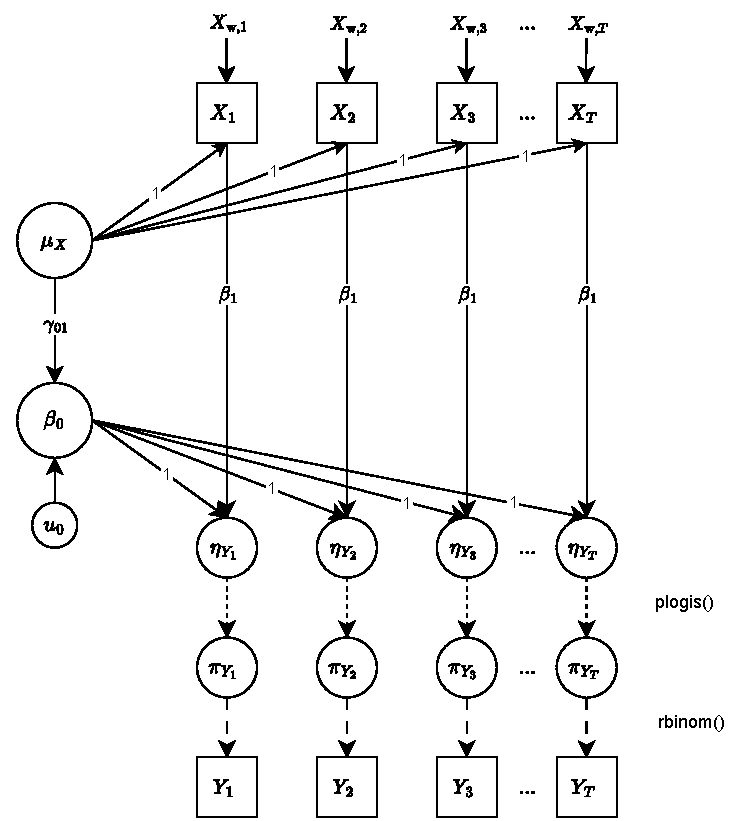
\includegraphics[width=\linewidth, height=8cm, keepaspectratio]{Figures/pathdiagrams-contxbiny.drawio.pdf}
%             \caption{Continuous X and Binary Y}\label{fig:path-contxbiny}
%         \end{subfigure}
%     \end{minipage}

%     % \vskip 1em

%     % Bottom row
%     \begin{minipage}[t]{.49\linewidth}
%         \centering
%         \begin{subfigure}[b]{\linewidth}
%             \centering
%             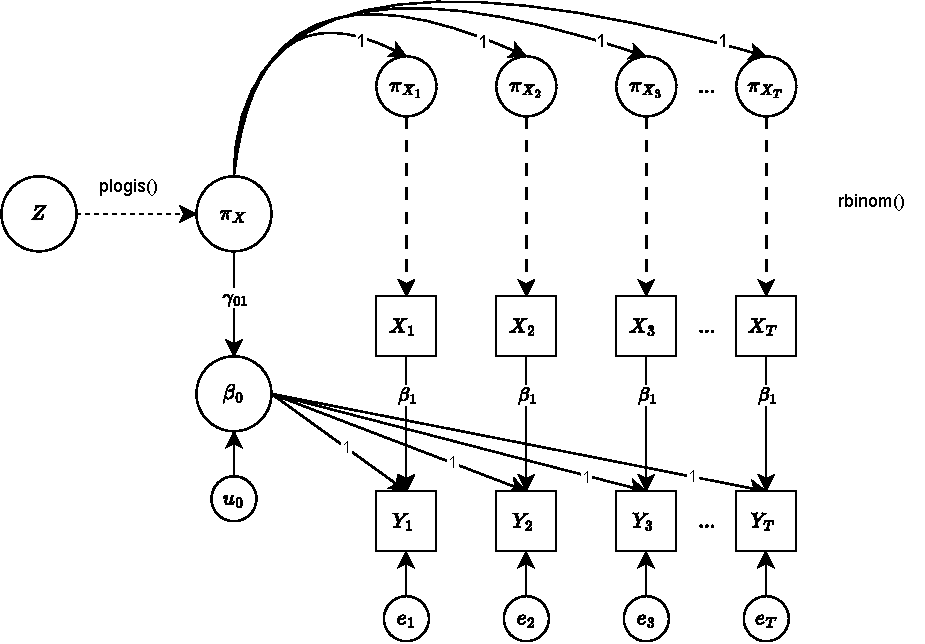
\includegraphics[width=\linewidth, height=8cm, keepaspectratio]{Figures/pathdiagrams-binxconty.drawio.pdf}
%             \caption{Binary X and Continuous Y}\label{fig:path-binxconty}
%         \end{subfigure}
%     \end{minipage}
%     \hfill
%     \begin{minipage}[t]{.49\linewidth}
%         \centering
%         \begin{subfigure}[b]{\linewidth}
%             \centering
%             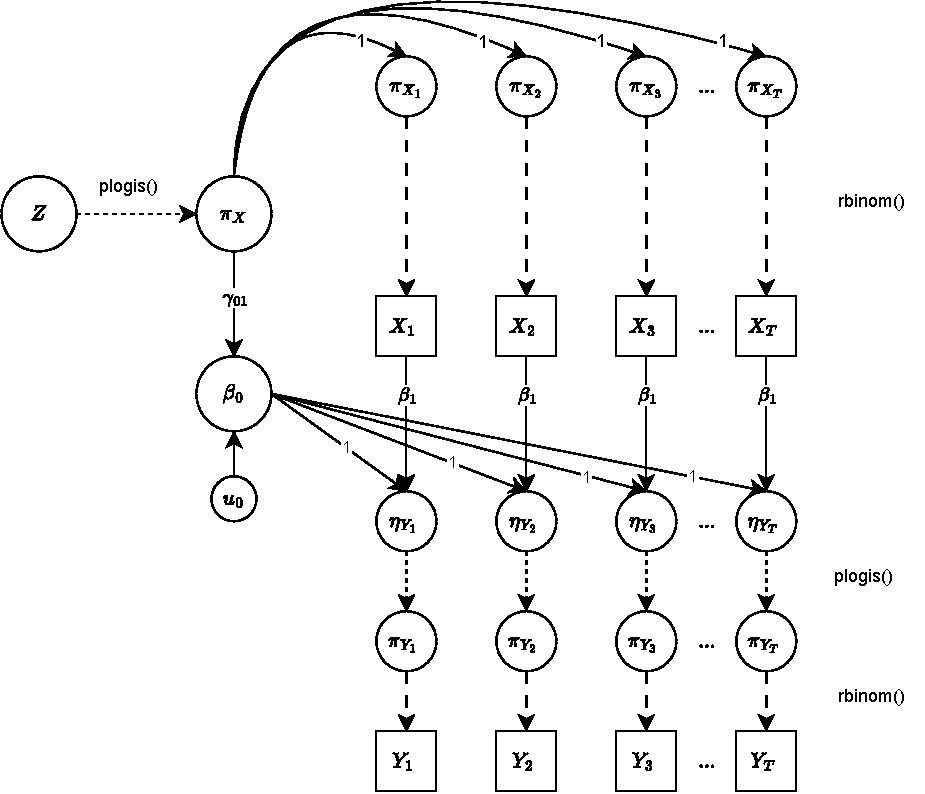
\includegraphics[width=\linewidth, height=8cm, keepaspectratio]{Figures/pathdiagrams-binxy.drawio.pdf}
%             \caption{Binary X and Y}\label{fig:path-binxy}
%         \end{subfigure}
%     \end{minipage}
%     \vspace{-1cm}
%     \label{fig:path}
%     \begin{flushleft}
%     \begin{figurenote}
%     Circles represent latent variables, squares represent observed variables, and arrows indicate relationships. Solid arrows denote linear associations, with a coefficient of 1 indicating a one-to-one relationship. Dotted arrows represent logit transformations (\texttt{plogis} in \texttt{R}), and dashed arrows represent Bernoulli sampling based on the probability $\pi$ (\texttt{rbinom} in \texttt{R}).
%     \end{figurenote}
%     \end{flushleft}
% \end{center}

% \begin{center}
% \captionof{figure}{Path diagrams of Generative Models with Within-Person ($\beta_\text{w}$) and Contextual Effect ($\gamma_{01}$)}

% \begin{minipage}[t]{.49\linewidth}
%     \centering
%     \begin{subfigure}[b]{\linewidth}
%         \centering
%         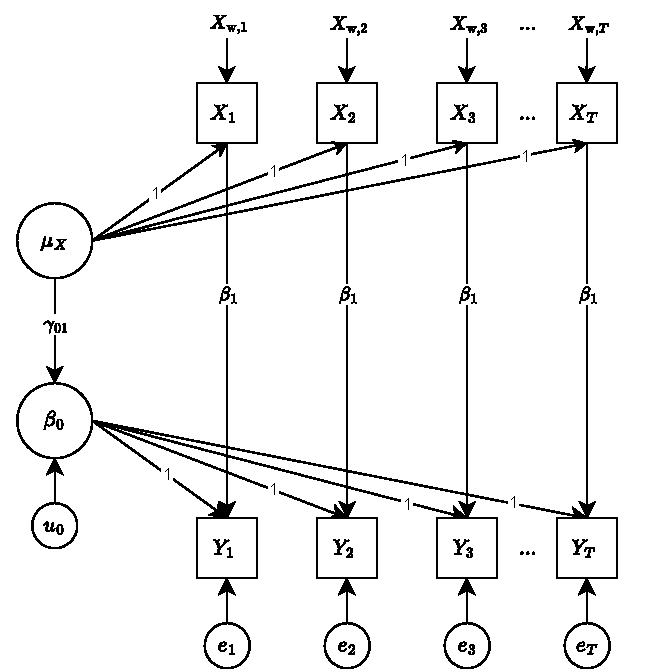
\includegraphics[width=\linewidth, height=8cm, keepaspectratio]{Figures/pathdiagrams-contxy.drawio.pdf}
%         \caption{Continuous X and Y}\label{fig:path-contxy}
%     \end{subfigure}
%     \vspace{1em}
%     \begin{subfigure}[b]{\linewidth}
%         \centering
%         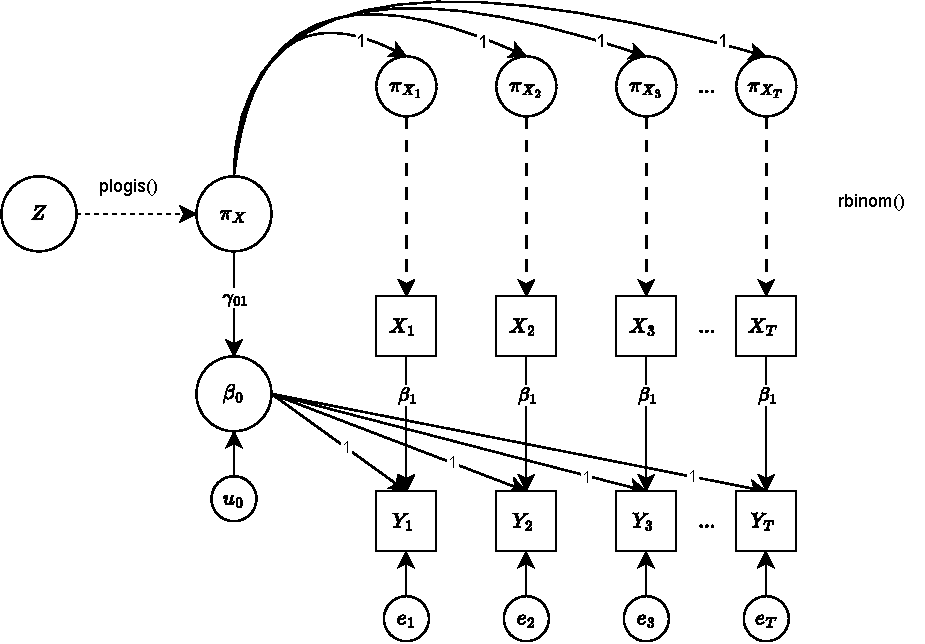
\includegraphics[width=\linewidth, height=8cm, keepaspectratio]{Figures/pathdiagrams-binxconty.drawio.pdf}
%         \caption{Binary X and Continuous Y}\label{fig:path-binxconty}
%     \end{subfigure}
% \end{minipage}
% \hfill
% \begin{minipage}[t]{.49\linewidth}
%     \centering
%     \begin{subfigure}[b]{\linewidth}
%         \centering
%         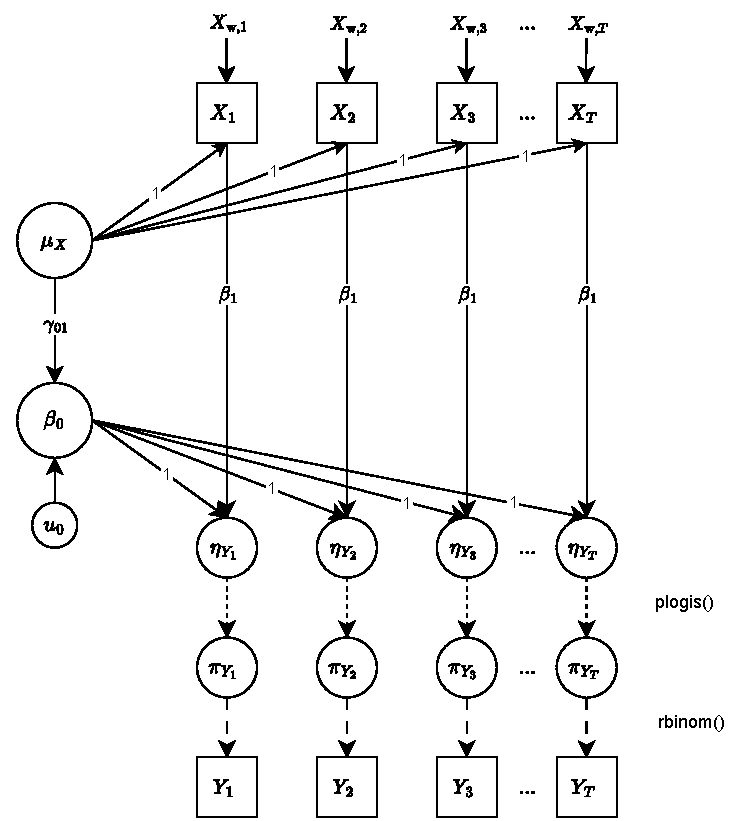
\includegraphics[width=\linewidth, height=8cm, keepaspectratio]{Figures/pathdiagrams-contxbiny.drawio.pdf}
%         \caption{Continuous X and Binary Y}\label{fig:path-contxbiny}
%     \end{subfigure}
%     \vspace{1em}
%     \begin{subfigure}[b]{\linewidth}
%         \centering
%         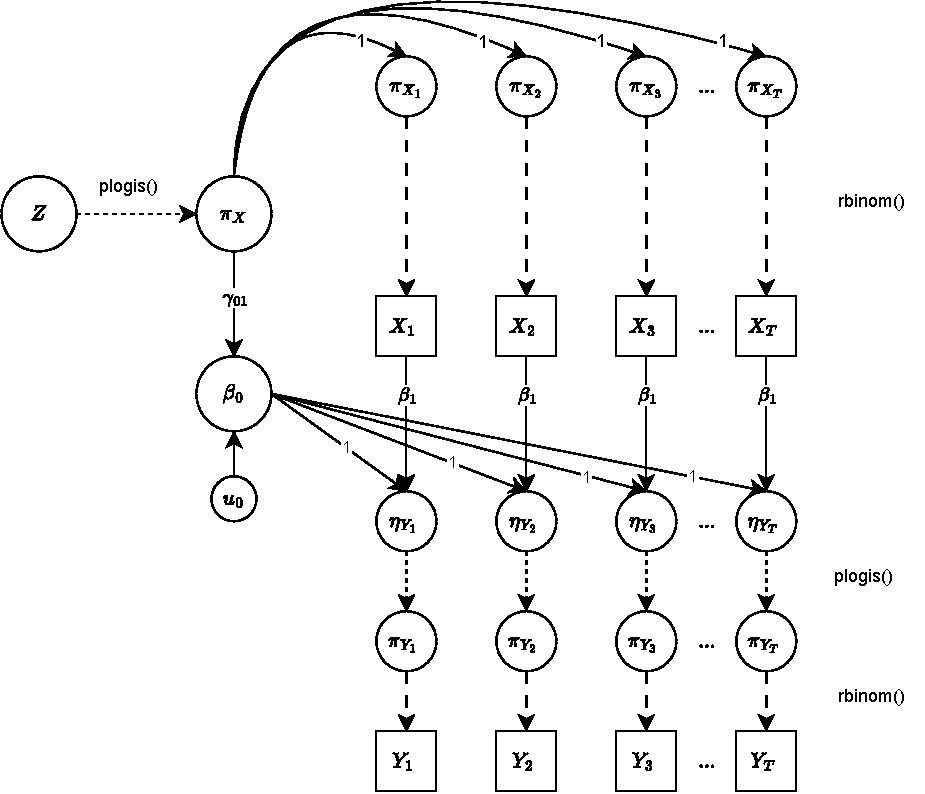
\includegraphics[width=\linewidth, height=8cm, keepaspectratio]{Figures/pathdiagrams-binxy.drawio.pdf}
%         \caption{Binary X and Y}\label{fig:path-binxy}
%     \end{subfigure}
% \end{minipage}

% \vspace{-0.5cm}
% \label{fig:path}

% \begin{flushleft}
% \begin{figurenote}
% Circles represent latent variables, squares represent observed variables, and arrows indicate relationships. Solid arrows denote linear associations, with a coefficient of 1 indicating a one-to-one relationship. Dotted arrows represent logit transformations (\texttt{plogis} in \texttt{R}), and dashed arrows represent Bernoulli sampling based on the probability $\pi$ (\texttt{rbinom} in \texttt{R}).
% \end{figurenote}
% \end{flushleft}
% \end{center}
